\section{Other systematics sources}
\label{sec:systematics}
% ---- ---- ---- ---- ---- ---- ---- ---- ---- ---- ---- ---- ---- ---- ---- ---- ---- ---- ---- ---- ---- ---- ----


\subsection{Jet energy scale}
% .... .... .... .... .... .... .... .... .... .... .... .... .... .... .... .... .... .... .... .... .... .... ....


To evaluate the uncertainty due to jet energy scale in events with the
topology of this analysis, we reconstruct the hadronic W candidate
from an almost pure top data control sample.  A semileptonic top
sample is a good proxy for signal for the purposes of this study,
since the top quark pairs are produced by gluon fusion and decay to
two W bosons. These semileptonic top events are selected by requiring
exactly four jets in the event, out of which two are b-tagged and the
other two are anti-btagged. The hadronic W candidates are formed from
two anti-btagged jets.  The invariant mass of the hadronic W
candidates in the combined channels is shown in
Figure~\ref{fig:topw:muel}, for data and Monte Carlo, together with a
gaussian fit on the peak of each distribution.  The relative
difference between the gaussian means in data and Monte Carlo is used
as jet energy scale uncertainty, and propagated through the template
fits in the backgrounds, as well as to the signal shapes in the limit
setting. These results for 2012 are consistent with those found for
2011, when the typical effect was found to be of the order of less
than a percent.
%% as an example of signal shapes shown in Fig.~\ref{fig:sys:jesonsignal}.

\begin{figure}[htb] 
  {\centering
    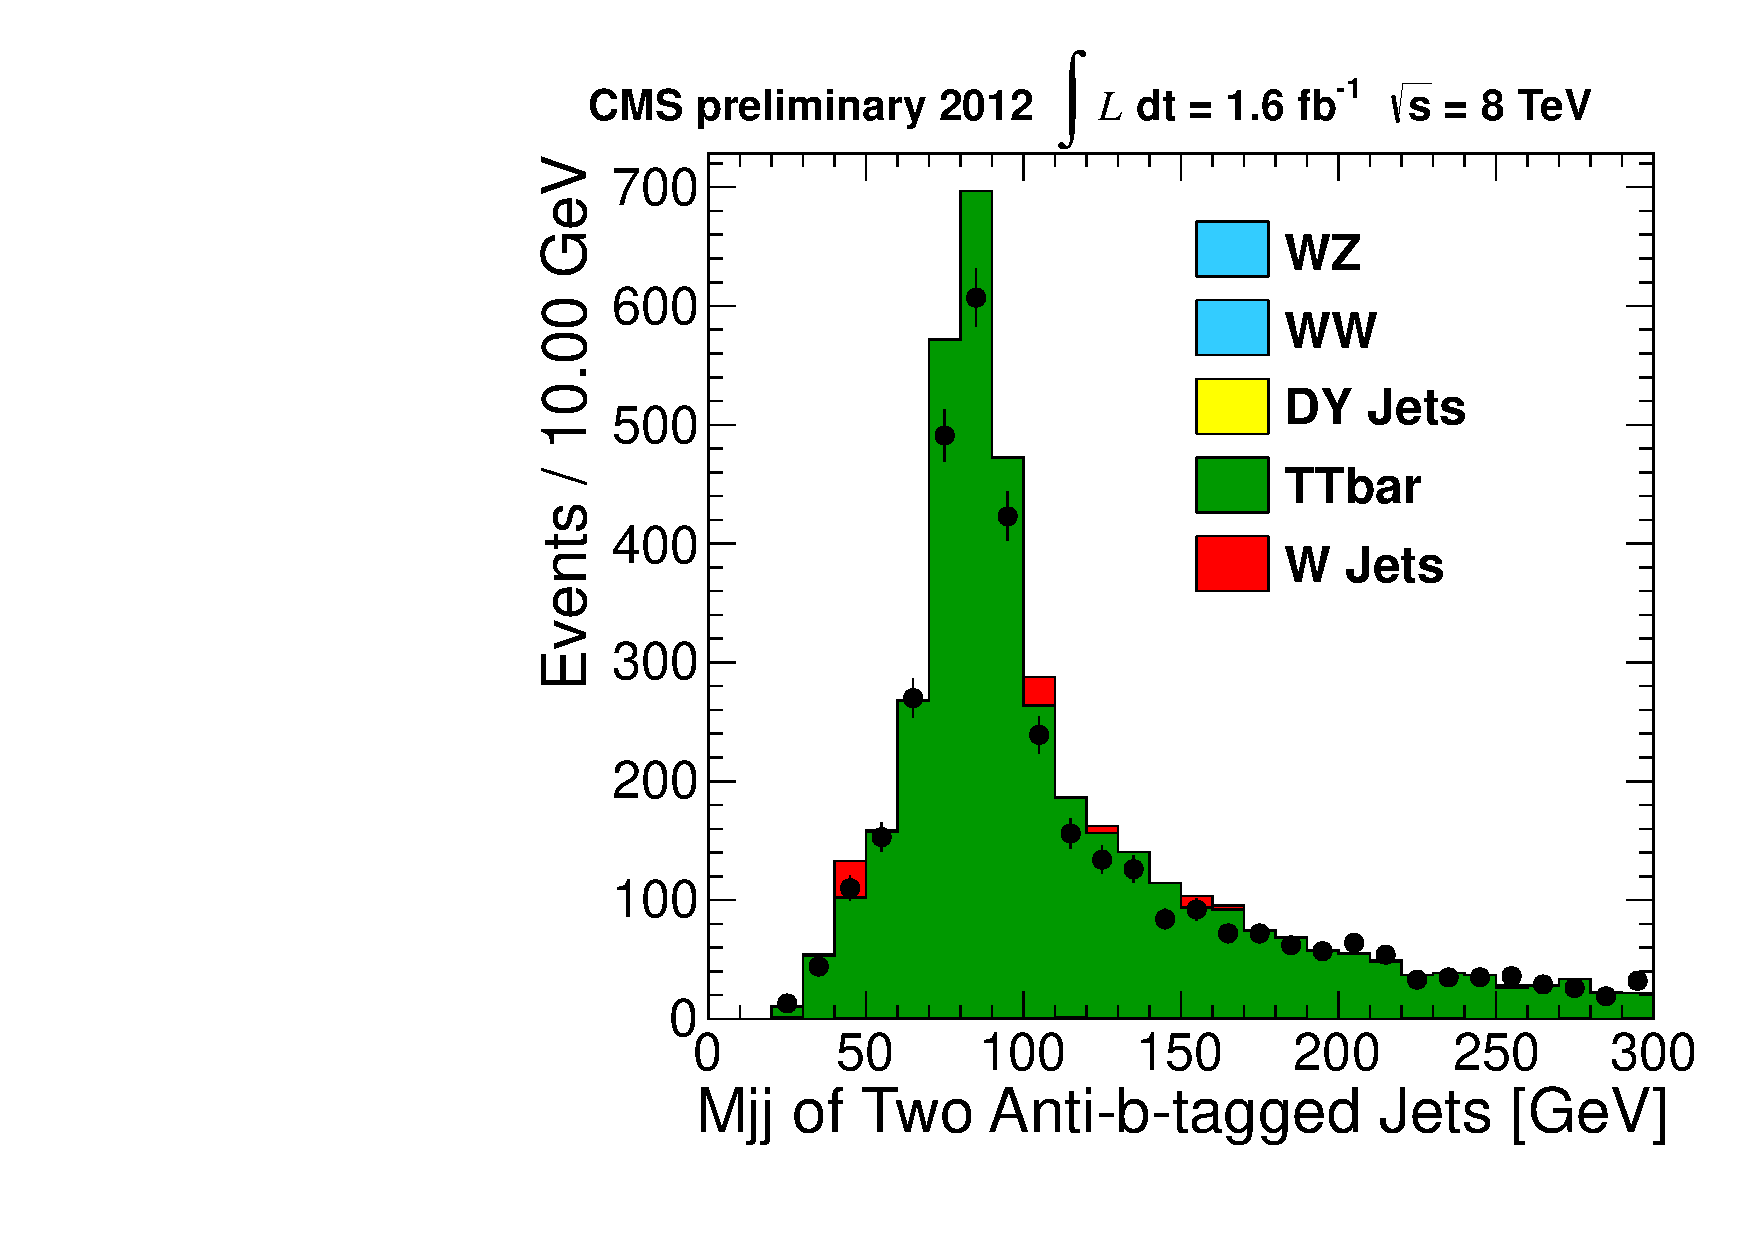
\includegraphics[width=0.325\textwidth]{plots/2012_JES/top_overlap_muel.pdf}
    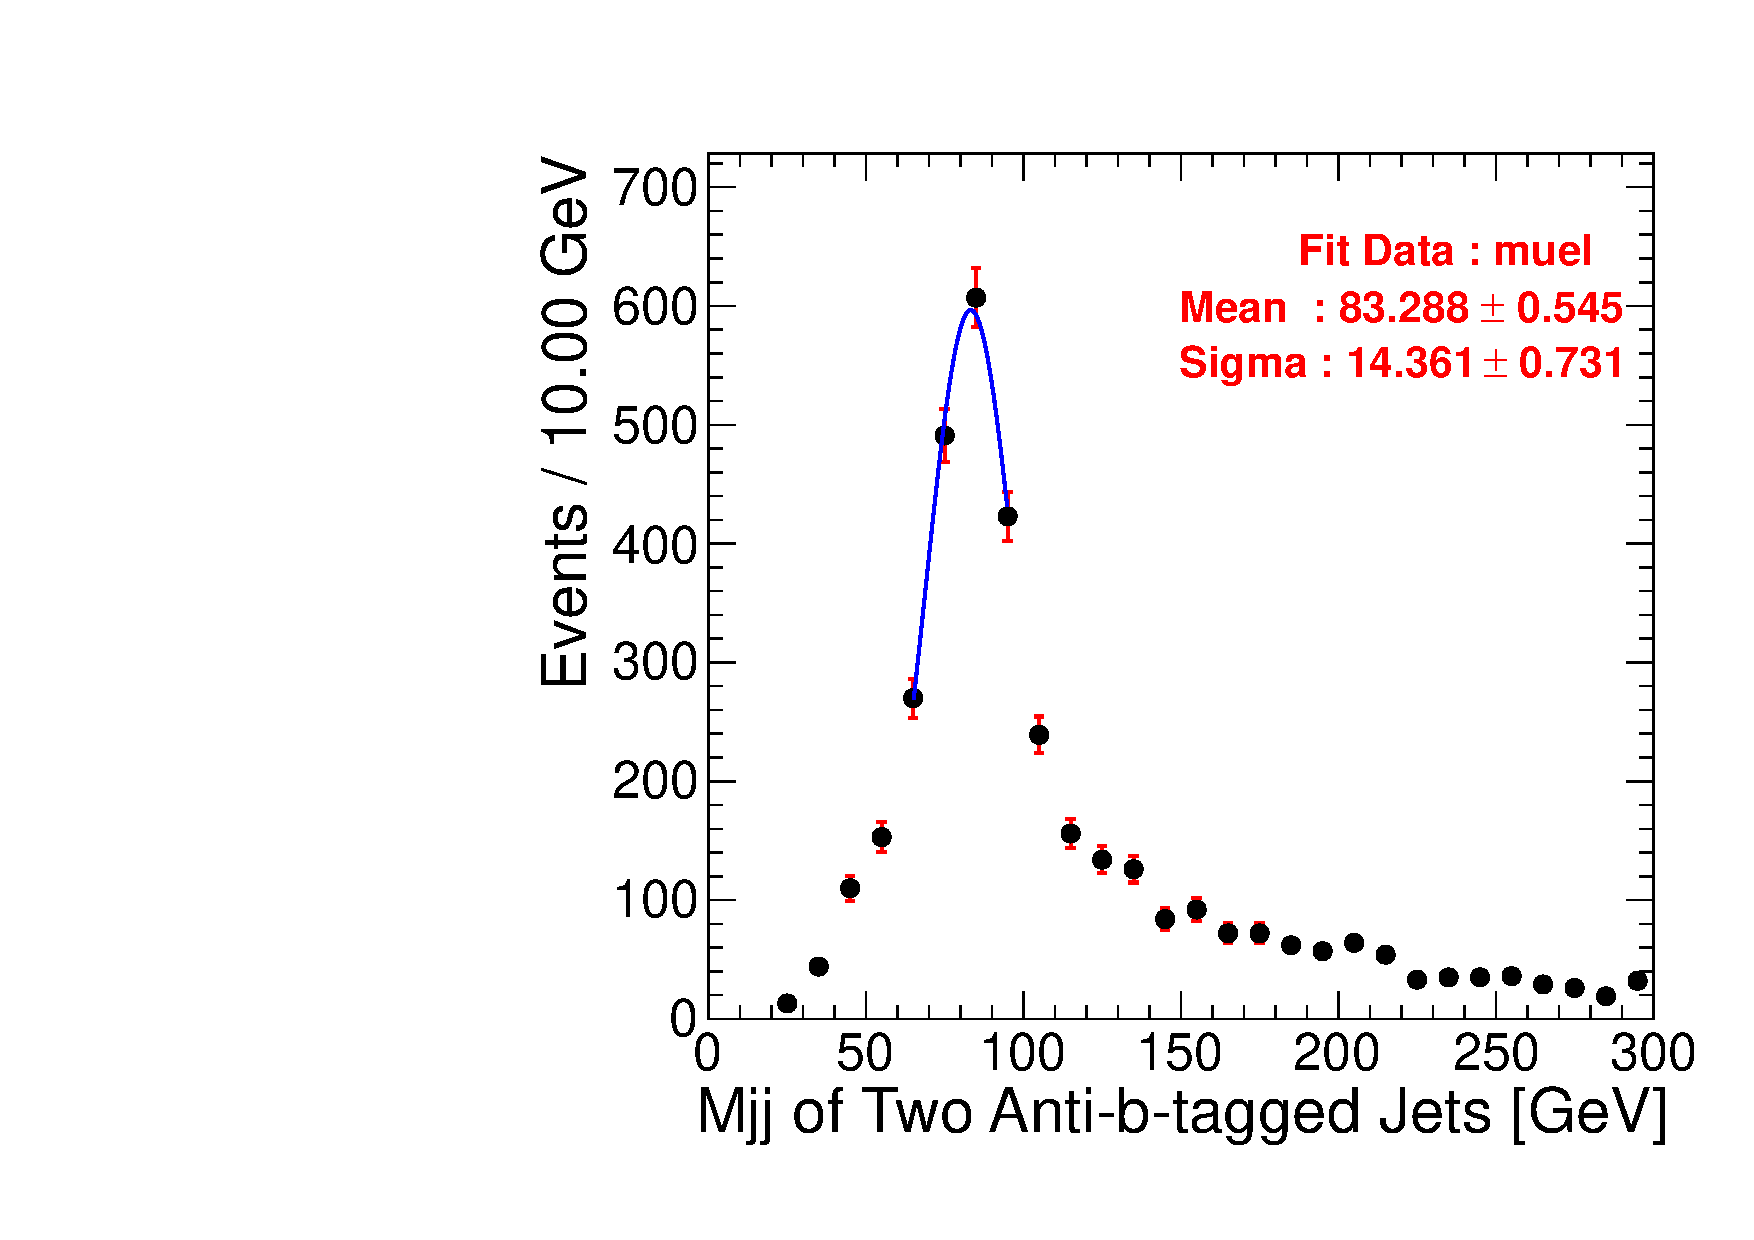
\includegraphics[width=0.325\textwidth]{plots/2012_JES/top_data_fit_muel.pdf}
    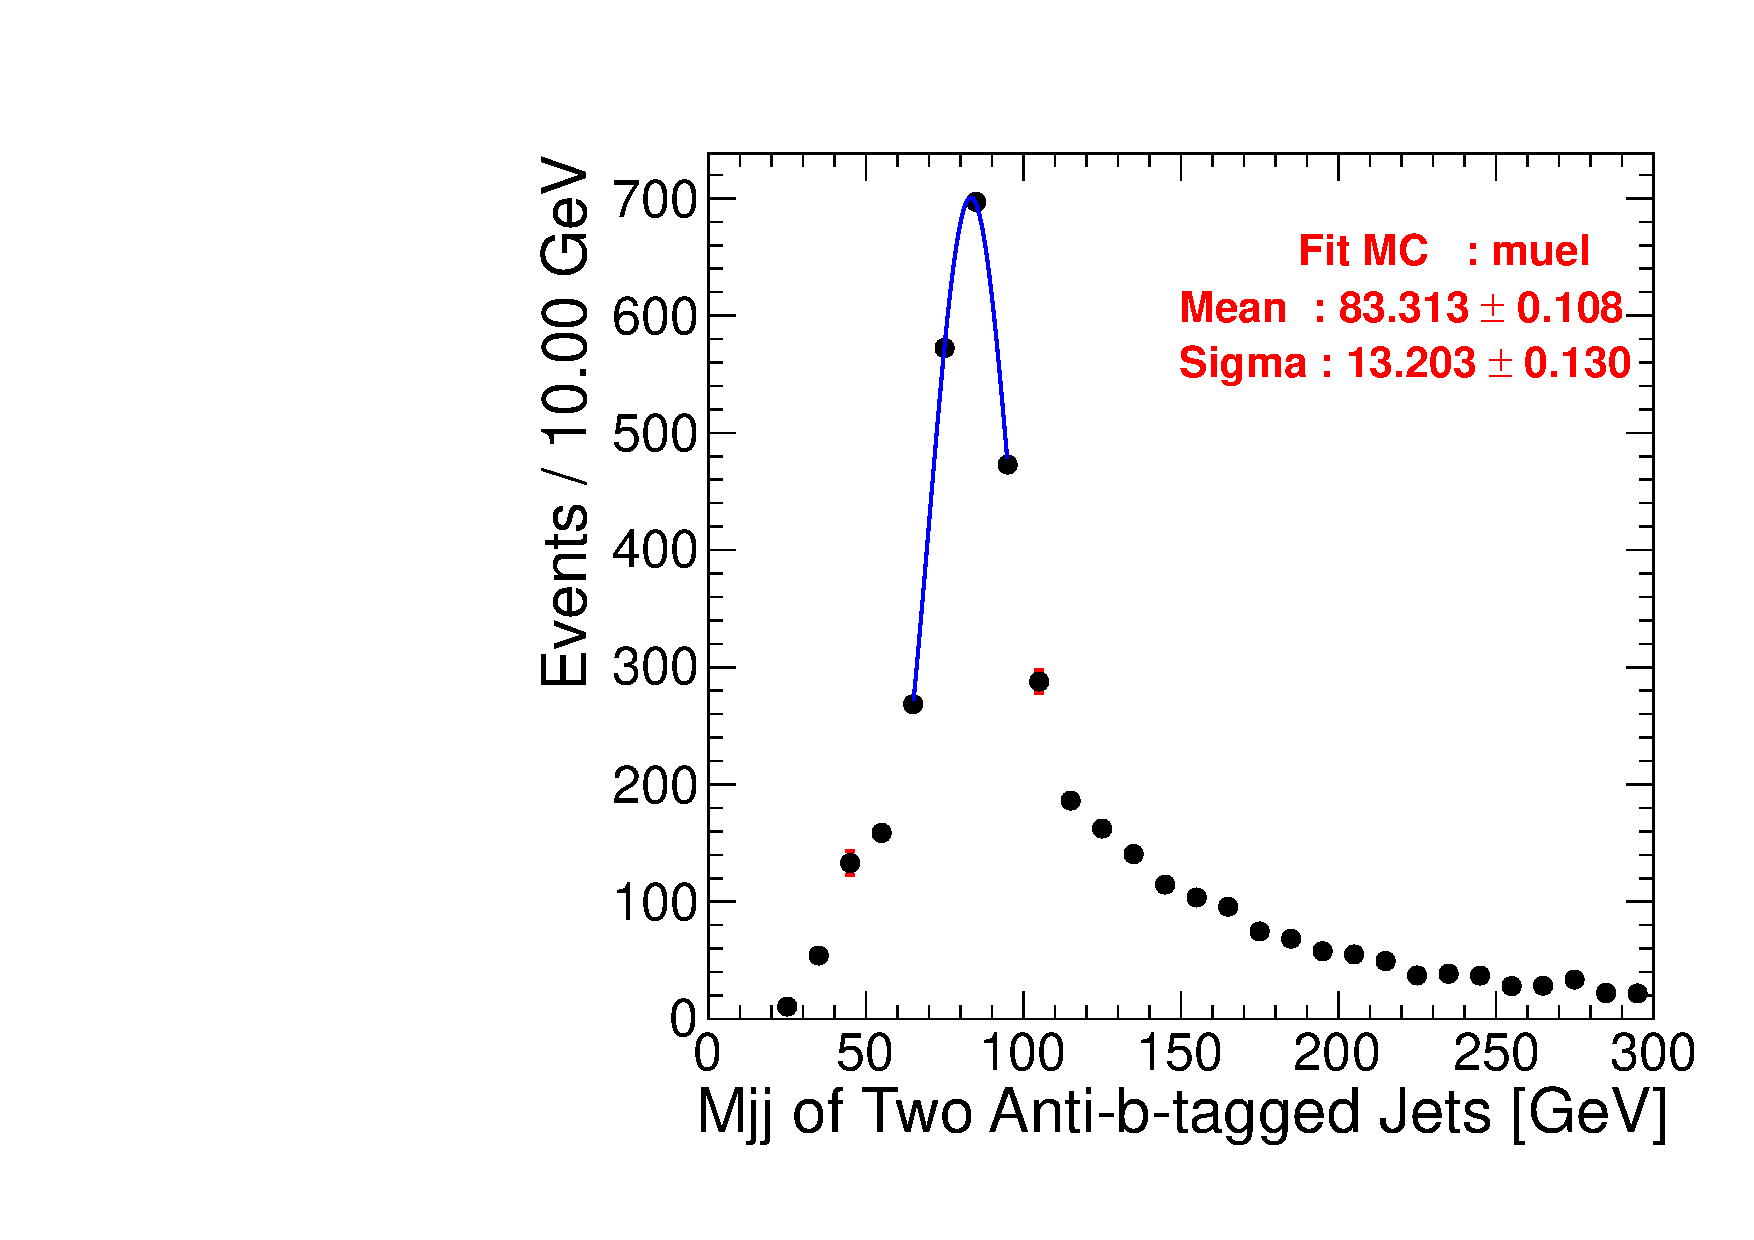
\includegraphics[width=0.325\textwidth]{plots/2012_JES/top_mc_fit_muel.pdf}
    \caption{The invariant mass distribution of the hadronic 
      W candidates in the semileptonic top sample (electron and 
      muon combined). 
      The left plot shows good agreement between the data and MC. 
      We fit the distribution with a Gaussian and extract the peak
      location for the data (middle) and MC (right).}
    \label{fig:topw:muel}}
\end{figure}

%% \begin{figure}[htb]
%%   \centering
%%   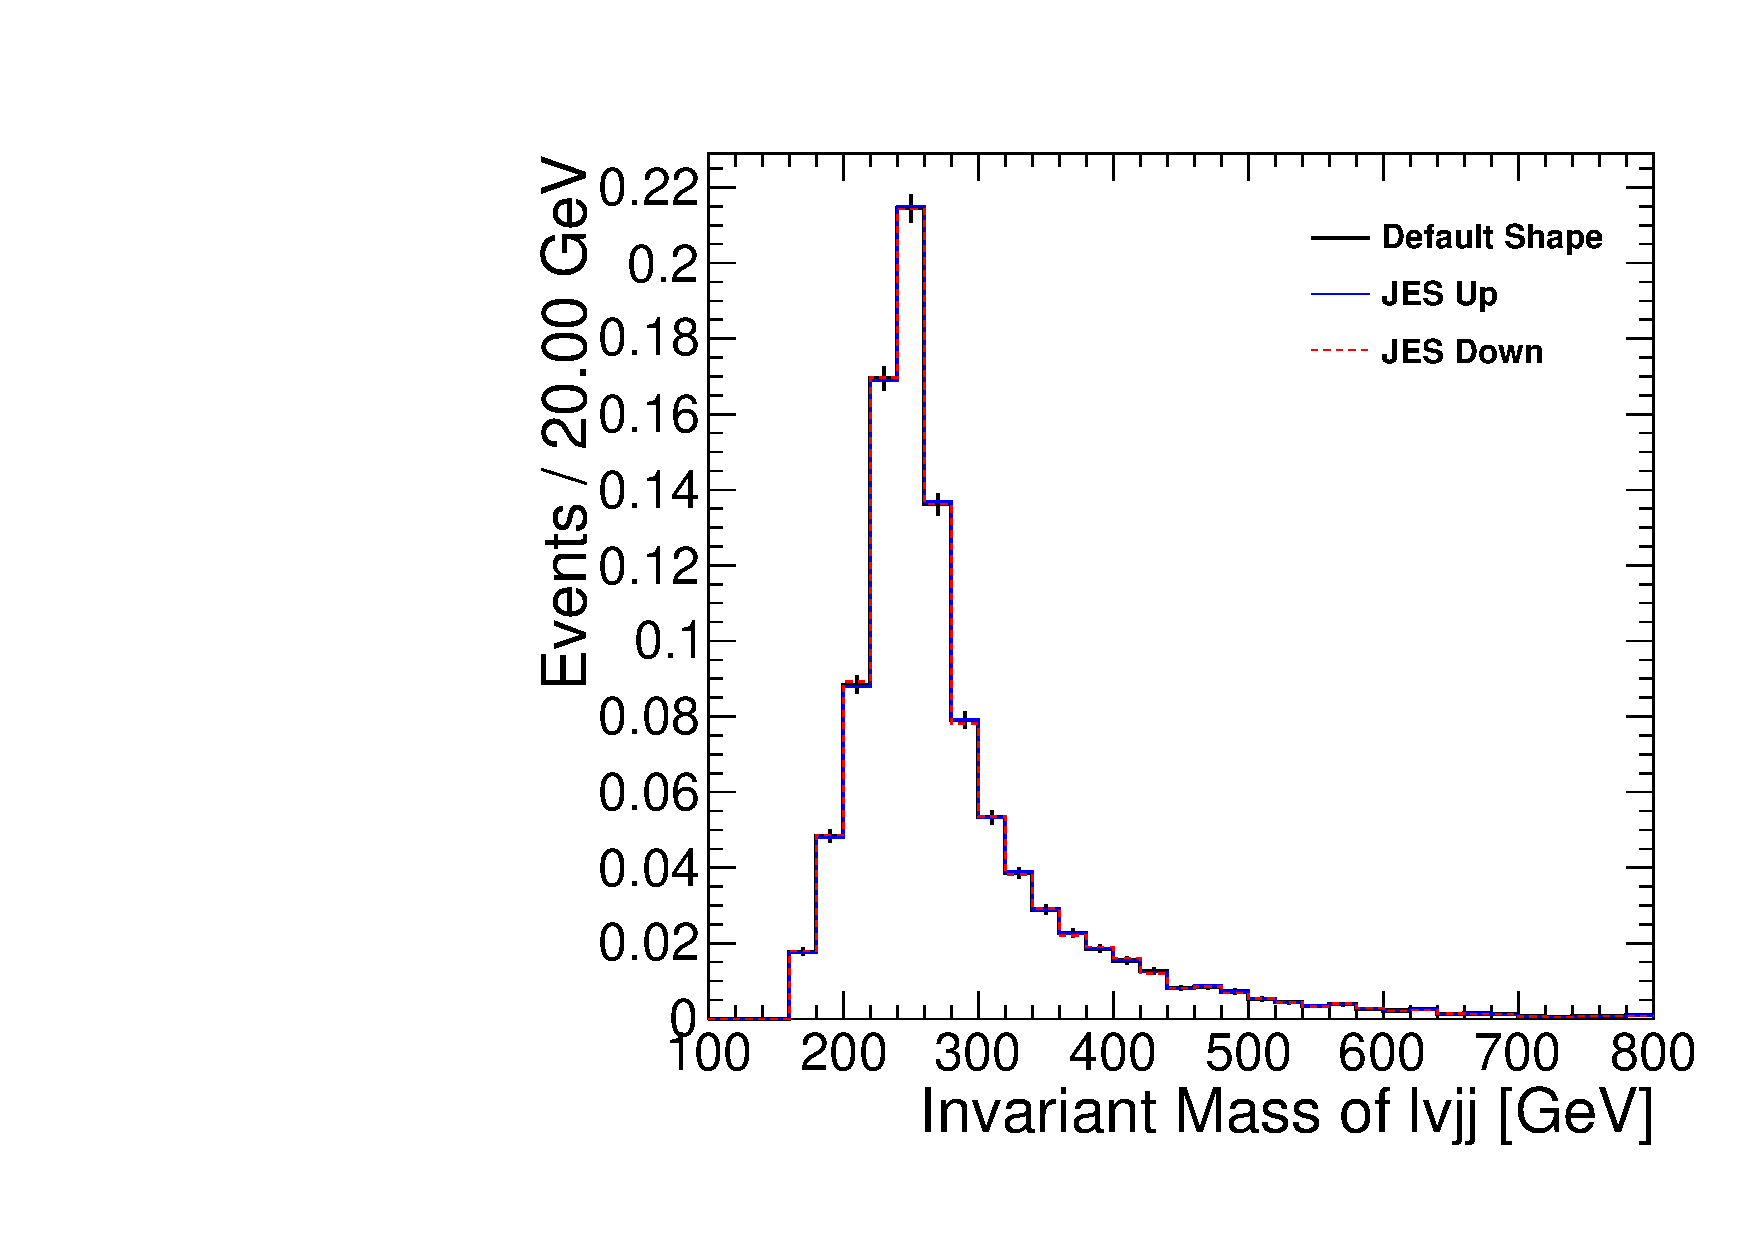
\includegraphics[width=0.49\textwidth]{plots/anaexample/sys-JES-mlvjj-mH250.pdf}
%%   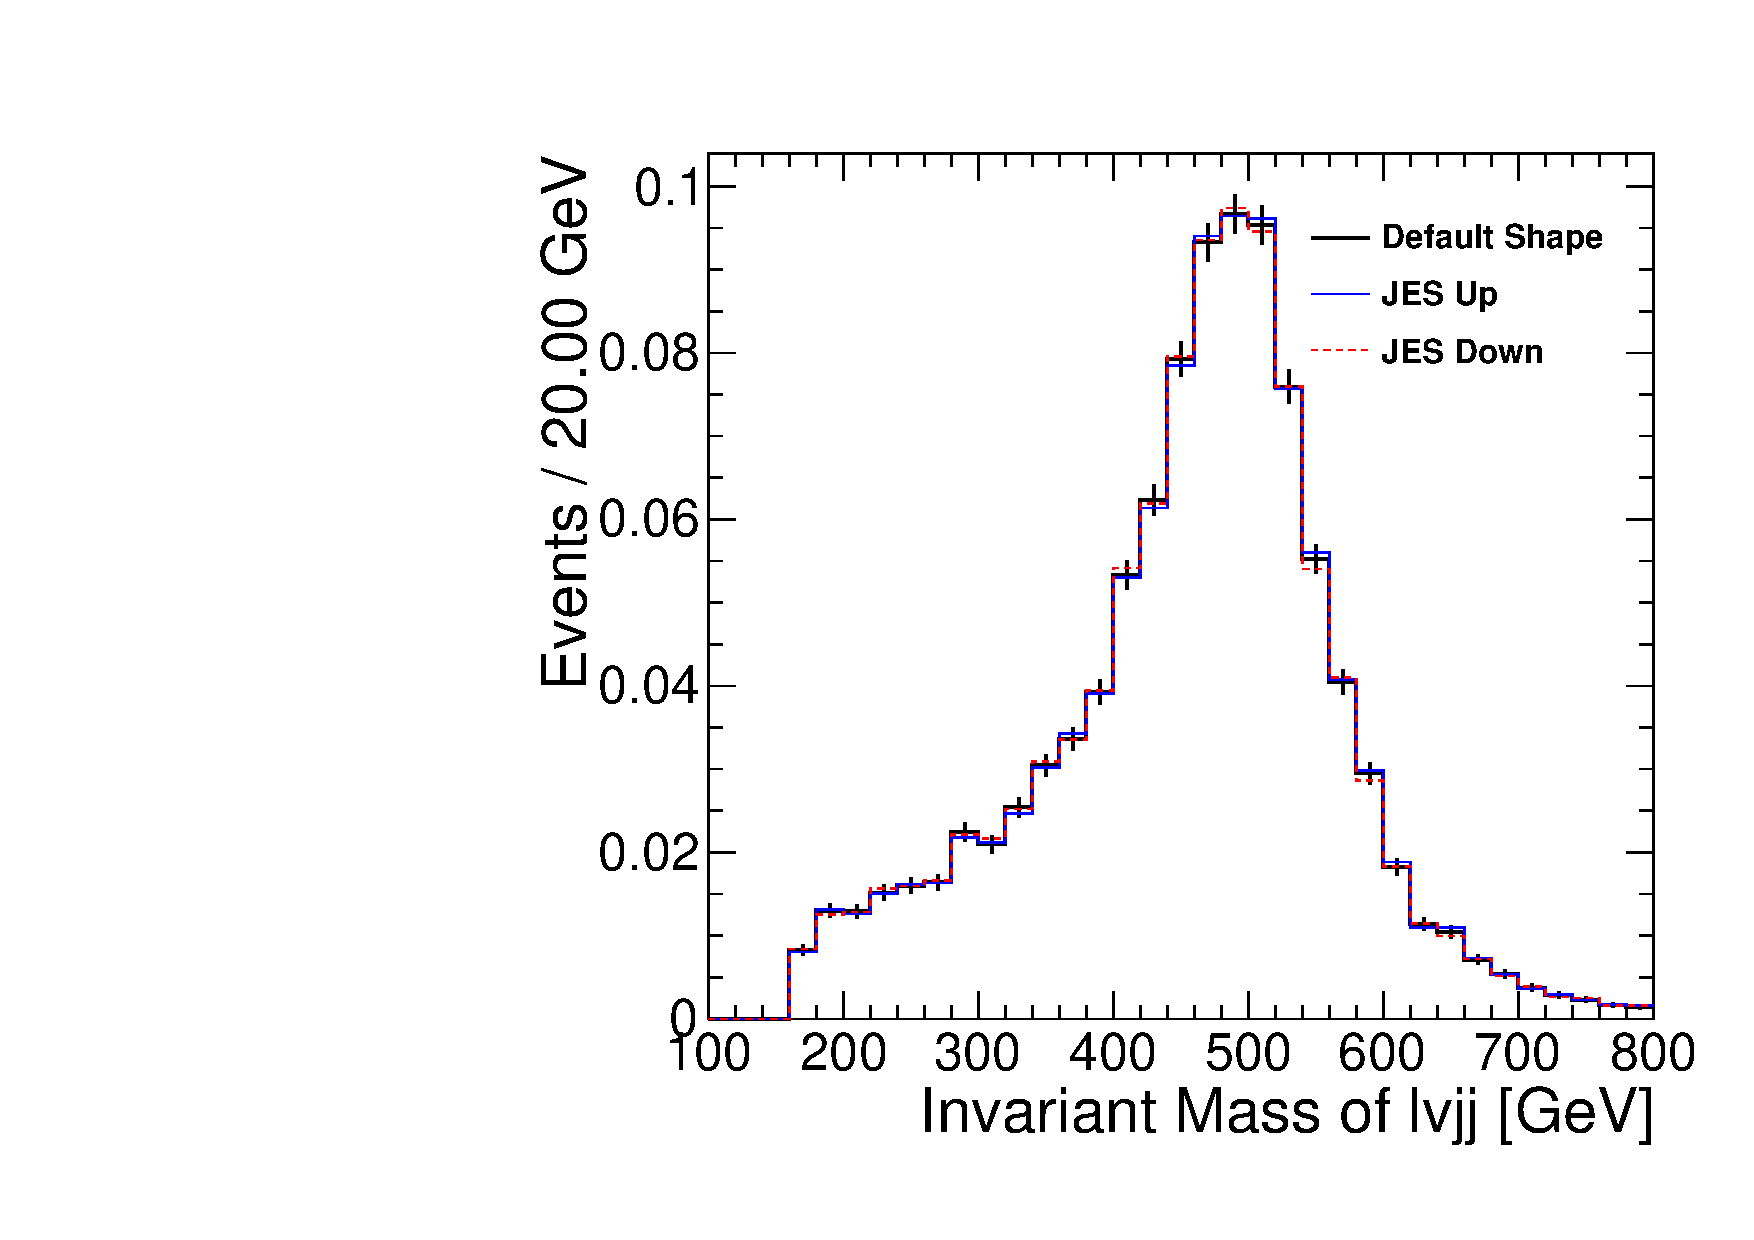
\includegraphics[width=0.49\textwidth]{plots/anaexample/sys-JES-mlvjj-mH500.pdf}
%%   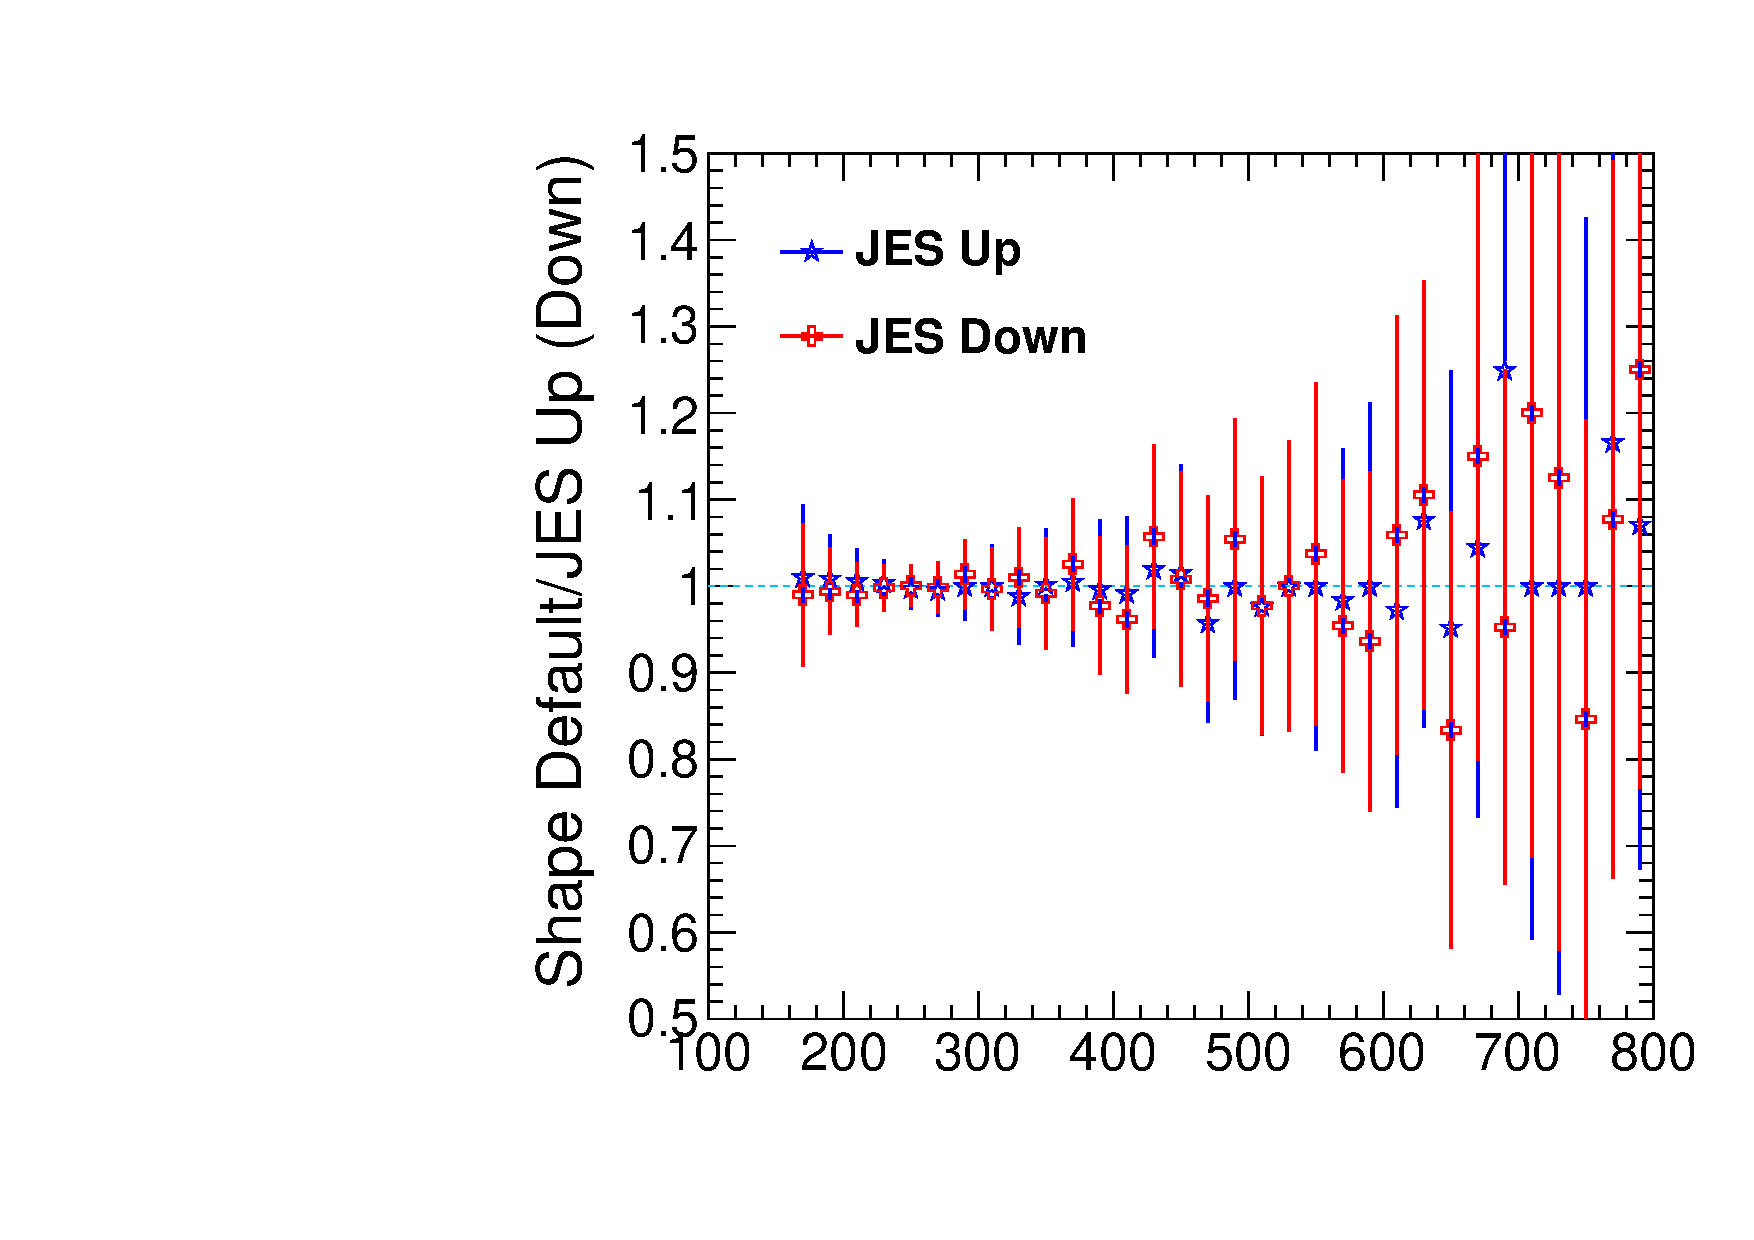
\includegraphics[width=0.49\textwidth]{plots/anaexample/sys-JES-ratio-mH250.pdf}
%%   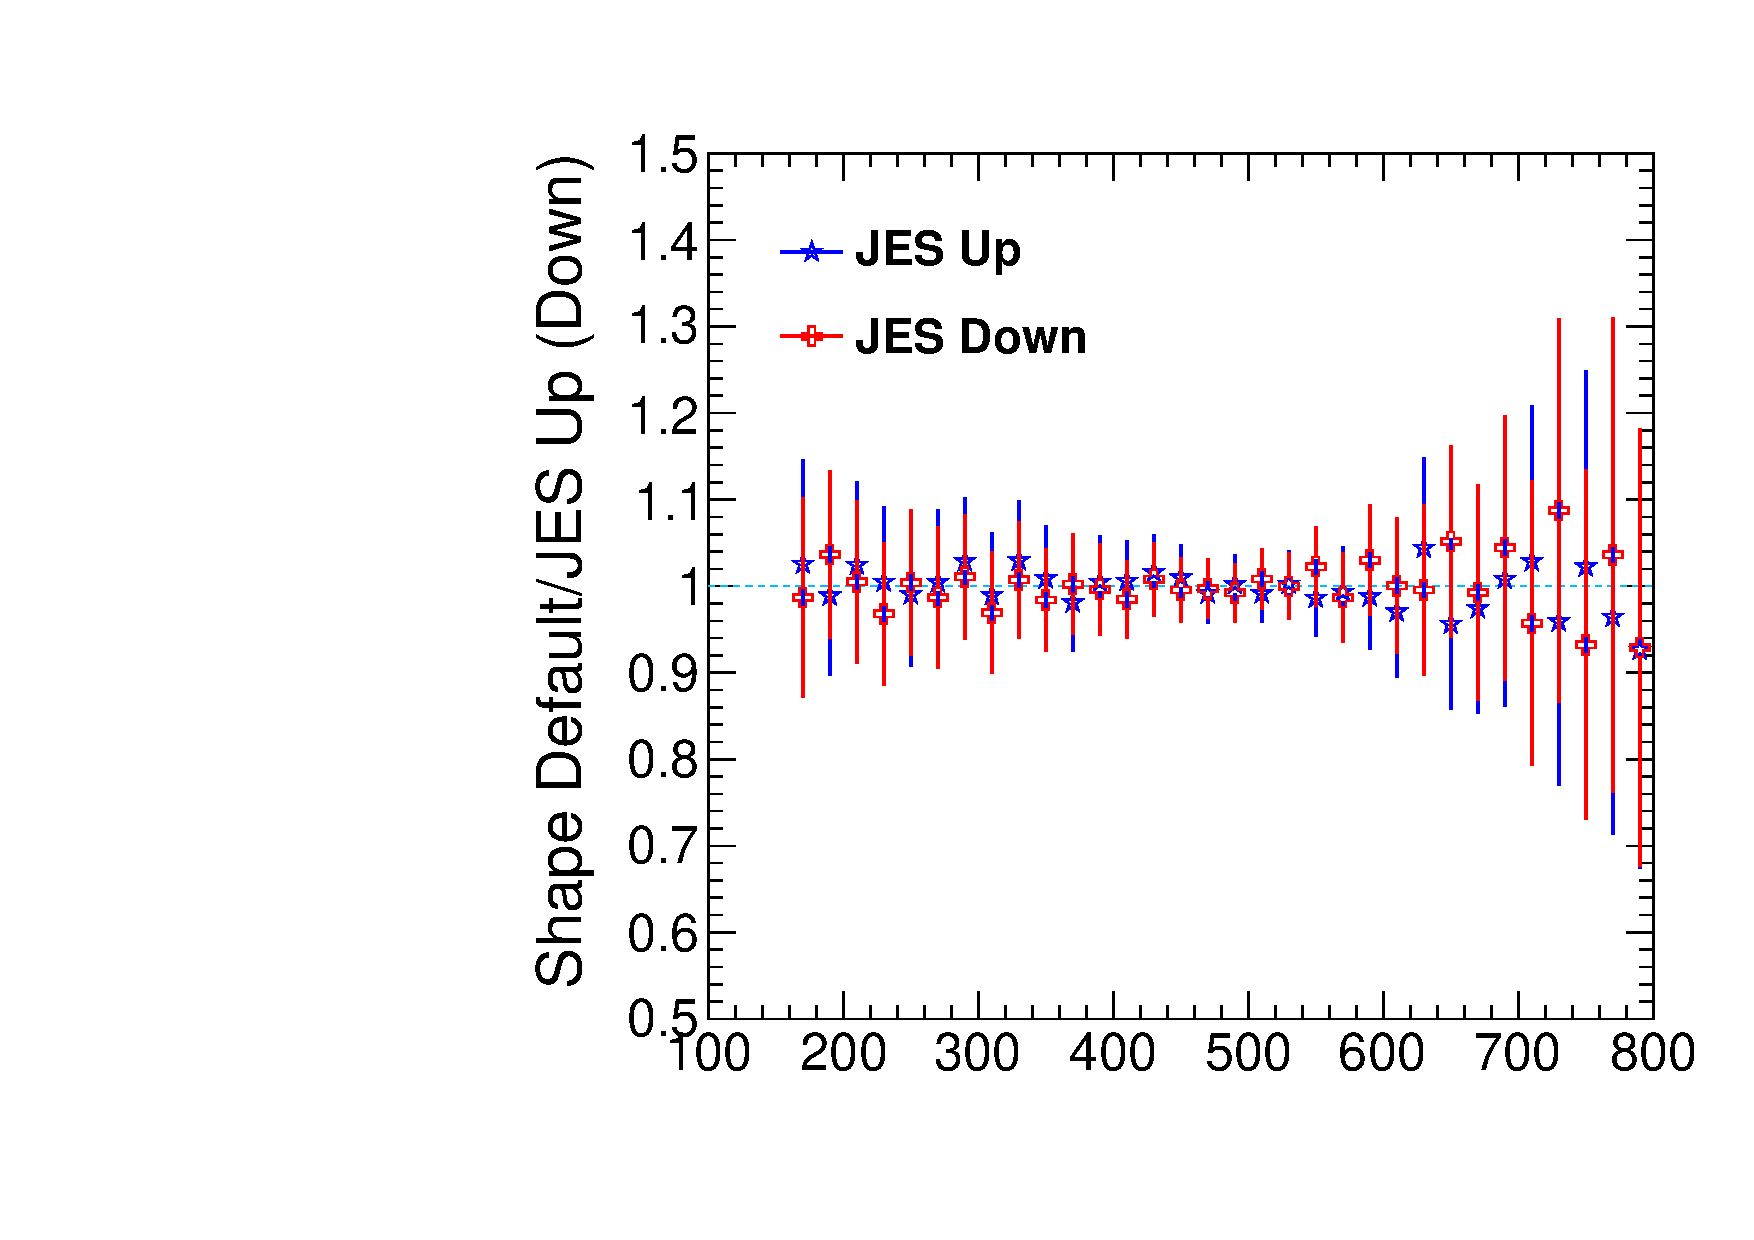
\includegraphics[width=0.49\textwidth]{plots/anaexample/sys-JES-ratio-mH500.pdf}
%%   \caption{\label{fig:sys:jesonsignal}The Higgs signal shape
%%     comparison between normal shape and the shape by shifting JES
%%     up/down by 0.5\%. The left plots are for Higgs mass 250~GeV and
%%     the right plots are for Higgs mass 500~GeV.}
%% \end{figure}

\subsection{Final selection efficiency on signal}
\label{sec:mvaseleffunc}

The systematic associated with the efficiency on the final selection
of the MVA output
%% and quark-gluon likelihood
is studied by using the same
top pair events as described above.  There is reasonable agreement
between the Monte Carlo and the data for the top sample. The
differences in selection efficiency are used to measure the potential
error in the signal efficiency for each mass point / channel
combination. The uncertainty is then taken as
\[
 100\% \times (1 - \frac{\epsilon_{data}}{\epsilon_{MC}}).
\]

The distribution of measured uncertainties per mass point/channel
combination is shown in Fig.~\ref{fig:sys:sigseleffuncdist}. The measured
efficiency uncertainties varied from less than 1\% to 10\%.
We therefore conservatively take 10\%
as the signal selection efficiency uncertainty for all channels and
mass points.
We verified that
this conservative selection had no significant impact on the final
expected limit.

\begin{figure}[htb]
\center
%%\subfigure[
  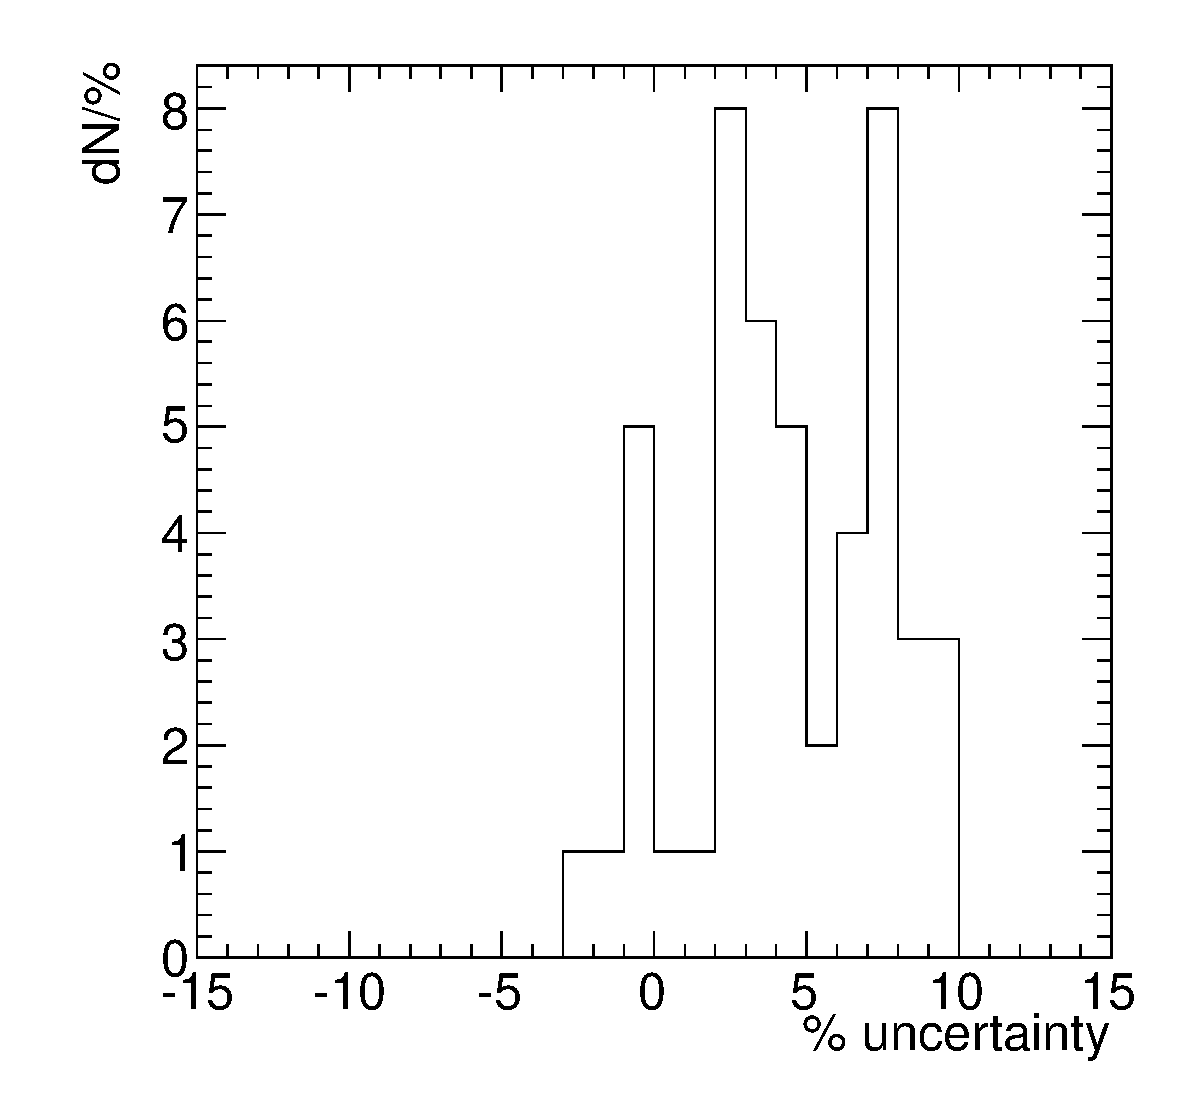
\includegraphics[width=0.49\textwidth]{plots/anaexample/sigseleffuncdist.pdf}
%% \subfigure[\label{fig:sys:sigseleffxcheck}] {
%%   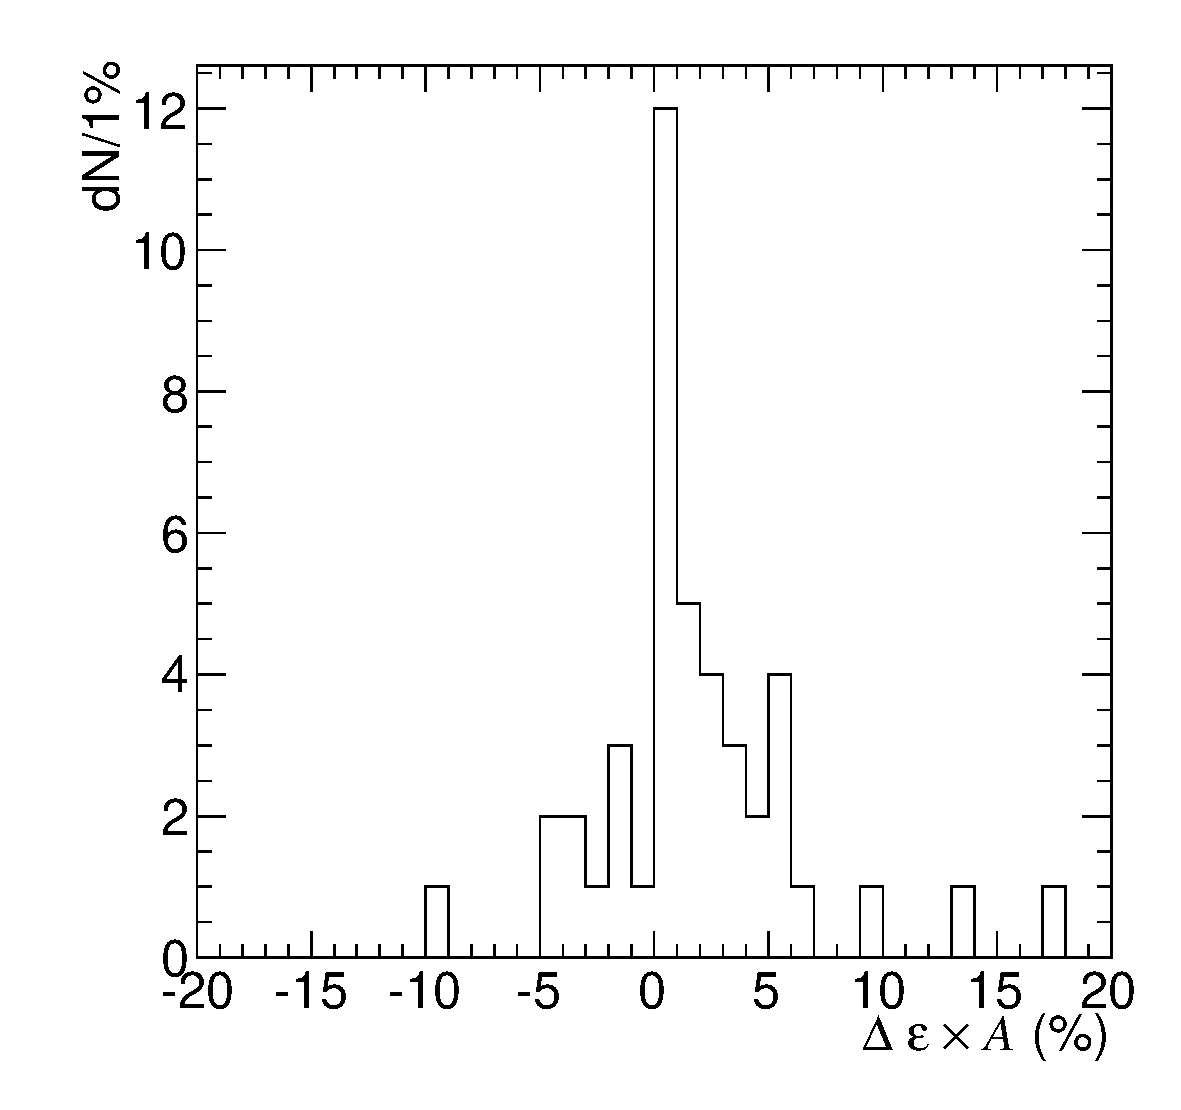
\includegraphics[width=0.49\textwidth]{plots/anaexample/sigseleffxcheckrewght.pdf}
%% }
  \caption{The distribution of measured uncertainties on signal
selection efficiency, one entry per channel/mass point
combination.
%% The uncertainties for high masses, for which the
%% quark-gluon likelihood discriminant is applied in addition to the MVA
%% discriminant, are shown in color.
%% b) The distribution, one entry per
%% channel/mass point, of the change in acceptance times efficiency
%% caused by reweighting the signal MC with the MVA output. The spread
%% is consistent with the quoted systematic.
}
\label{fig:sys:sigseleffuncdist}
\end{figure}

\subsection{Lepton selection and trigger efficiency}
%%.... .... .... .... .... .... .... .... .... .... .... .... .... .... .... .... .... .... .... .... .... .... ....
%%The lepton trigger and selection is common among several CMS analyses and 
%%we benefit from common studies based on tag-and-probe techniques. 
%%
Systematic uncertainties in the trigger efficiencies
are of the order of 1\%. Systematic uncertainties in the lepton reconstruction
and identification efficiency scale factors are of the order of 2\%. These uncertainties
are accounted for in the final systematics that are input to the limit setter.

\subsection{MET uncertainty}
% .... .... .... .... .... .... .... .... .... .... .... .... .... .... .... .... .... .... .... .... .... .... ....

MET directly affects our signal acceptance. 
The uncertainty prescription is discussed in Ref.~\cite{met}.
%https://twiki.cern.ch/twiki/bin/viewauth/CMS/MissingETUncertaintyPrescription
In addition, the MET distribution in the data is $\simeq$3\% wider 
than the MC, and placing a hard MET$>30.0$ cut creates an uncertainty. 
We estimate it by smearing the MET for each event by a Gaussian with 
a $\sigma =0.03*$MET and observing how many events pass the cut. 
Specifically, (Events Passing After Smearing)/(Events Passing Before Smearing) 
=0.998 for both muons and electrons.


\subsection{Pile-up model}
% .... .... .... .... .... .... .... .... .... .... .... .... .... .... .... .... .... .... .... .... .... .... ....


The average number of pile-up interaction in a given bunch crossing
BX$_{i}$ is given by the following formula:
\begin{equation}
N_{i} = \frac{\mathcal{L} \cdot \sigma_{\textnormal{min. bias}}}{\nu_{\textnormal{orbit}}},
\end{equation}
where $\mathcal{L}$ is the instantaneous luminosity,
$\sigma_{\textnormal{min. bias}}$ is the cross-section of minimum bias
interactions and $\nu_{\textnormal{orbit}}$ is the LHC orbit frequency
(11246~Hz).  Source of uncertainties in the estimation of the number
of pile-up interactions in data then come from the uncertainty on the
luminosity, currently $\textnormal{syst}_{\textnormal{lumi}}=4.4\%$ and
the uncertainty on the minimum-bias cross-section. We have adopted
$\sigma_{\textnormal{min. bias}}=69.3$~mb.

A total variation of 5\% in the number of interactions was propagated to the
re-weighting procedure for signal samples, and the obtained variation
in the signal yield is used as systematics on the signal. The typical
effect is less than a percent and therefore neglected.


\subsection{Cross-section prediction}
% .... .... .... .... .... .... .... .... .... .... .... .... .... .... .... .... .... .... .... .... .... .... ....


As of this writing, the inclusive cross-sections used for the Higgs
signal at 8~TeV center-of-mass energy have been calculated by the
Higgs Cross Section Working Group
\cite{LHCHiggsCrossSectionWorkingGroup:2011ti} for the
gluon-gluon fusion process, and have been used in the limits
extraction, together with their uncertainties, which are of the
order of 15-20\%. Equivalent cross-sections and uncertainties for the
vector boson fusion process have not yet been calculated, so the values
for 7~TeV center-of-mass energy scaled by a factor of 1.3 are used in
their place.

In addition, the acceptance effect due to the PDF choice has been
studyied by following the PDF4LHC recipe, that considers as
uncertainty the envelope of the error calculated for three sets of
PDFs \cite{Whalley:2005nh}, namely CT10, NNPDF and MSTW.
Table~\ref{tab:signalPDF} shows the values obtained.  For the purposes
of the limits calculation, these systematics are added in quadrature
to the inclusive cross-section uncertainties.
%
\begin{table}[h!t]
  \caption{Acceptance uncertainty related to the PDFs variation, 
           for the signal rate, as a function of the mass hypothesis.}
  \label{tab:signalPDF}
  \begin{center}
    \begin{tabular}{lc|lc}
      \hline
      \multicolumn{2}{c|}{ggF} & \multicolumn{2}{c}{VBF} \\
      \hline
      $m_{H}$ &  unc.   & $m_{H}$ &  unc.  \\
      \hline
       170  &  2.0\%  &  170  &  2.0\% \\ %FIXME conservative  
       180  &  2.0\%  &  180  &  2.0\% \\ %FIXME conservative  
       190  &  2.0\%  &  190  &  2.0\% \\ %FIXME conservative  
       200  &  2.0\%  &  200  &  2.0\% \\ %FIXME conservative  
       250  &  1.5\%  &  250  &  1.1\% \\  
       300  &  2.0\%  &  300  &  0.9\% \\  
       350  &  2.2\%  &  350  &  0.8\% \\  
       400  &  2.4\%  &  400  &  0.6\% \\  
       450  &  2.7\%  &  450  &  0.7\% \\  
       500  &  2.9\%  &  500  &  0.9\% \\  
       550  &  3.2\%  &  550  &  0.9\% \\  
       600  &  3.6\%  &  600  &  0.7\% \\  
      \hline
    \end{tabular}
  \end{center}
\end{table}

%% Eventually, an uncertainty is considered, in the case of gluon fusion
%% production, to account for the limitation of the narrow Higgs width
%% approximation in the Higgs simulation, and for the effect of
%% interference with Standard Model (SM) backgrounds.  The value used is
%% parametrized as a function of the Higgs mass as $150 \times m_H^3
%% [\%]$ where $m_H$ is expressed in TeV
%% \cite{Passarino:2010qk,Campbell:2011cu,Anastasiou:2011pi}.

Finally, there are uncertainties associated with the exclusive jet
binning used in this analysis. A detailed description of the source of
this uncertainty and how to calculate it is described in
\cite{cite:combine} Appendix C.  For this analysis we adopt the
numbers calculated by the $H\rightarrow WW\rightarrow 2\ell 2\nu$
group (\cite{cite:higgs2l2nu} Section~8.1).

\subsection{LHC luminosity}
% .... .... .... .... .... .... .... .... .... .... .... .... .... .... .... .... .... .... .... .... .... .... ....

A luminosity uncertainty of 4.4\% is applied to signal processesd~\cite{lumiPAS}.

\subsection{Uncertainties related to interference }

Appendix~\ref{sec:HHIntf} describes the procedure for reweighting
signal samples to correct for the effect of interference between the
signal and the SM $gg \to WW$ production process. It also describes
the recipe for estimating the uncertainty band associated with the
weight factors. 

Since the effect of interference enhances the cross-section of the
signal, this uncertainty band propagates through the analysis in two
ways: it changes the efficiency of the analysis selections on signal
events, and it alters the shape of the signal invariant mass
distribution that is used to set the upper limit. These are treated
simultaneously by applying the up- and down-fluctuated weights to the
signal distribution, in the same way that the nominal weights are
applied. These alternative shapes are also propagated to the limit setter.
Figure~\ref{fig:sigshapeintfunc} shows an example of this variation
for a Higgs mass of 600~\GeV, for which, of all the mass hypotheses
considered, the effect is largest.

\begin{figure}[t!]
  \begin{center}
    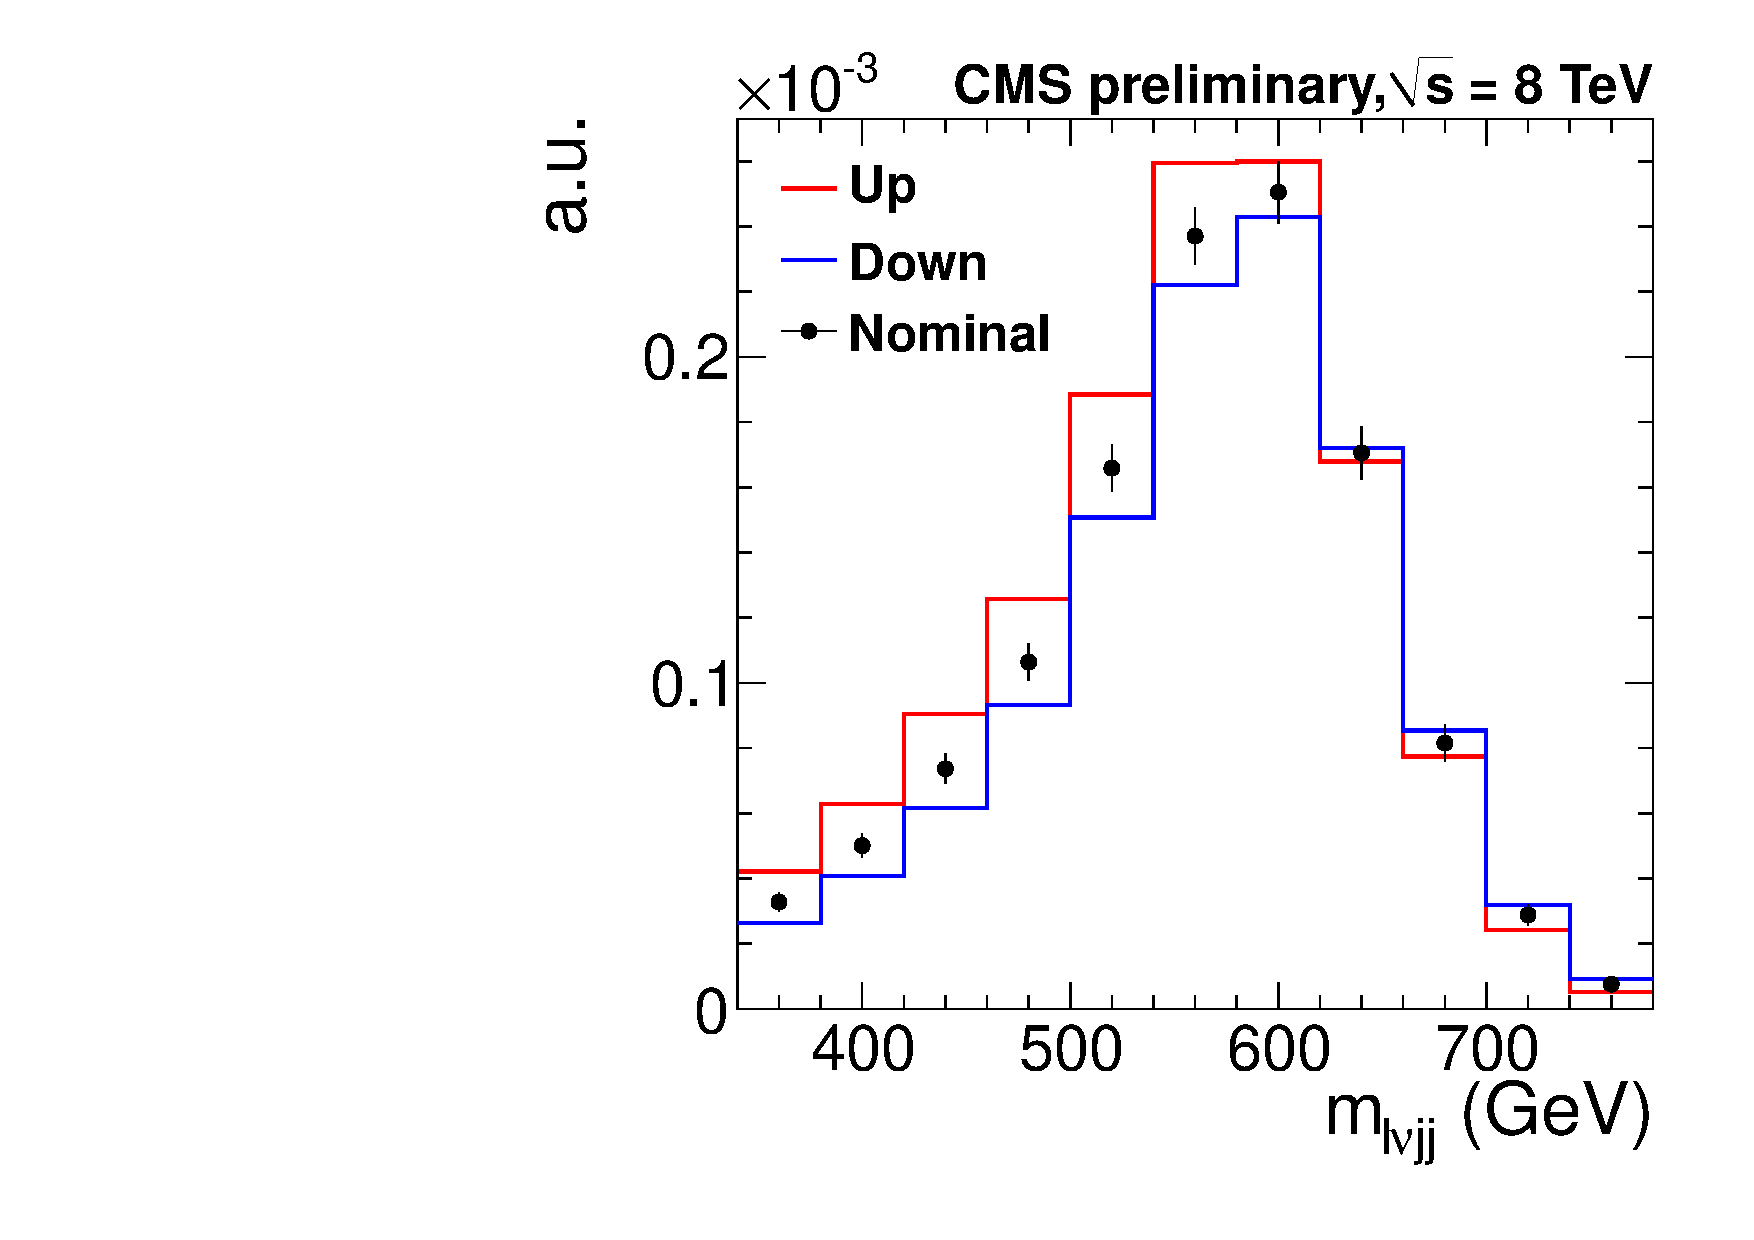
\includegraphics[width=0.5\linewidth]{plots/anaexample/H600_Muon_2jets_Signal_Shape.pdf}
  \caption{The shape variation for the signal $m_{\ell\nu jj}$ distribution,
  for a Higgs mass of 600~\GeV, muon 2-jet category. }
  \label{fig:sigshapeintfunc}
  \end{center}
\end{figure}

% .... .... .... .... .... .... .... .... .... .... .... .... .... .... .... .... .... .... .... .... .... .... ....

%%%%%%%%%%%%%%%%%%%%%%%%%%%%%%%%%%%%%%%%%%%%
\subsection{W+jets shape}
\label{sec:syst_mlvjj}
%%%%%%%%%%%%%%%%%%%%%%%%%%%%%%%%%%%%%%%%%%%%%
The $m_{\ell\nu jj}$ shape for W+jets events is taken from the data
sidebands. To get a smooth shape we parametrize this data-driven
shape using an exponential function. The decay parameter of this
parameterization has an associated error with it. We vary the
parameter up and down to get shape variations on the W+jets shape.
The shapes that are produced corresponding to the different systematic
variations on the parameters are propagated to the limit setting as a
systematic error.

The uncertainty on the $\alpha$ parameter used to combine the two
$m_{jj}$ sidebands would also constitute a variation in shape.  We
propagate the errors on alpha to the W+jets shape and combine its
effects on the shape with the uncertainty of the shape that arose
from the statistical power of the sideband data samples.

%%%%%%%%%%%%%%%%%%%%%%%%%%%%%%%%%%%%%%%%%%%%
\subsection{Background normalization}
\label{sec:syst_mjj}
%%%%%%%%%%%%%%%%%%%%%%%%%%%%%%%%%%%%%%%%%%%%%

The errors for the total background normalization are derived from the
unbinned maximum likelihood fit on the dijet invariant mass described
in Section~\ref{sec:mjjfitfornormal}. The non-Poisson fractional errors for
the 48 mass/lepton flavor/jet bin combinations are shown in
Table~\ref{tab:sys:normerrs}.  These are taken as a systematic
uncertainty on the background normalization in the signal region.

We compute these errors as
\[
\text{non-Poisson fractional error} \equiv \frac{\sqrt{\sigma_{N_\text{bkg}}^2-N_\text{bkg}}}{N_\text{bkg}}
\]
Poisson errors are included in the limit setting package.  We include
this additional systematic error which propagates additional
statistical errors derived in the dijet mass fit that are above and
beyond the Poisson errors alone.

\begin{table}[htb]
  \caption{Systematic uncertainties on the total background normalization.}
  \label{tab:sys:normerrs}
  \begin{center}
    \begin{tabular}{l|c|c|c|c} 
      \hline \hline
      $m_{\textnormal{H}}$  & electron 2-jet & electron 3-jet & muon 2-jet & muon 3-jet \\
      (\GeV) & (\%)  &  (\%) &  (\%) &  (\%)  \\ \hline
       170  &  0.2  &  0.3  &  0.2  &  0.2  \\
       180  &  0.5  &  0.3  &  0.5  &  0.2  \\
       190  &  0.3  &  0.3  &  0.3  &  0.2  \\
       200  &  0.6  &  0.4  &  0.4  &  0.3  \\
       250  &  0.3  &  0.4  &  0.3  &  0.3  \\
       300  &  0.3  &  0.5  &  0.3  &  0.7  \\
       350  &  0.9  &  0.8  &  2.5  &  1.3  \\
       400  &  0.4  &  0.8  &  0.5  &  0.8  \\
       450  &  0.6  &  2.9  &  0.7  &  1.8  \\
       500  &  0.9  &  1.9  &  1.0  &  1.7  \\
       550  &  0.9  &  4.1  &  1.2  &  1.9  \\
       600  &  1.6  &  0.9  &  1.3  &  1.6  \\
      \hline \hline
    \end{tabular}
  \end{center}
\end{table}

%  \subsection{Summary of systematic uncertainties}
%  % .... .... .... .... .... .... .... .... .... .... .... .... .... .... .... .... .... .... .... .... .... .... ....
%  
%  Table~\ref{tab:fitSystematics} summarizes all the sources of uncertainty considered.
%  %
%  \begin{table}[htb]
%    \begin{center}
%    \begin{tabular}{l|c|c}
%    \hline 
%    source                   &  impact on signal  &  impact on background \\
%    \hline
%    luminosity               &                    &            -          \\
%    cross-section            &                    &            -          \\
%    jet energy scale         &                    &                       \\
%    jet energy resolution    &                    &                       \\
%    unclustered met          &                    &                       \\
%    lepton energy scale      &                    &                       \\
%    trigger effiency         &                    &                       \\
%    lepton efficiency        &                    &                       \\
%    sideband fit             &         -          &                       \\
%    \hline
%    \end{tabular}
%    \end{center}
%    \caption{Sources of systematics considered in the fit analysis, with the corresponding value.}
%    \label{tab:fitSystematics}
%  \end{table}
%  %
%  
%  
